\chapter{Thời gian riêng, sự giãn thời gian và sự co độ dài}

Chúng ta sẽ thường chọn hệ đơn vị trong đó tốc độ ánh sáng là $c=1$. Trong các đơn vị đó, một năm thời gian và một năm ánh sáng khoảng cách có thể được so sánh trực tiếp, và các công thức dễ đọc hơn nhiều. Bất cứ khi nào $c$ có ý nghĩa vật lý, ta sẽ đưa nó trở lại. Phân tích thứ nguyên là đủ để xác định chỗ cần đặt nó.

\section{Lưới không-thời gian Galile}

Hãy bắt đầu với hệ thức tiền Einstein giữa một hệ quy chiếu đứng yên và một đoàn tàu chuyển động với vận tốc $v$ dọc theo trục $x$:
\begin{align}
x' &= x-vt, & t'&=t.
\label{eq:l4-galilean}
\end{align}
Phương trình thứ hai chứa giả thiết thời gian tuyệt đối của Newton. Mọi quan sát viên đều dùng cùng các lát cắt đồng thời, dù các gốc tọa độ không gian chuyển động tương đối với nhau.

Giả sử quan sát viên không dấu phẩy đứng bên đường ray còn quan sát viên có dấu phẩy ngồi trên tàu. Gốc tọa độ của tàu có $x'=0$, nên đường thế giới của nó trong các tọa độ không dấu phẩy là
\begin{equation}
x=vt.
\end{equation}
Đường nghiêng đó là trục $t'$. Trái lại, $t'=t$ nói rằng mọi đường có $t'$ không đổi đều chính là những đường ngang như các đường có $t$ không đổi.

\begin{figure}[H]
\centering
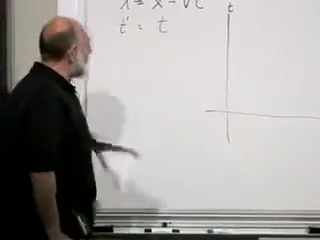
\includegraphics[width=0.72\textwidth]{lecture_04_figure_02.png}
\caption{Phép biến đổi Galile và lưới $t$-$x$ ban đầu. Gốc chuyển động sẽ vạch ra $x=vt$, trong khi hai hệ vẫn giữ chung các đường thời gian không đổi.}
\lectureframe{00:03:06}
\end{figure}

Giải phương trình~\eqref{eq:l4-galilean} theo các tọa độ không dấu phẩy, ta được
\begin{align}
x&=x'+vt'=x'+vt, & t&=t'.
\end{align}
Phép biến đổi nghịch đảo có cùng dạng, với $v$ được thay bằng $-v$. Nếu tàu chuyển động về phía trước so với ga, thì ga chuyển động lùi về phía sau so với tàu. Tính tương hỗ này vẫn còn trong thuyết tương đối hẹp, nhưng thời gian tuyệt đối thì không.

\section{Hiệu chỉnh Lorentz}

Các phép biến đổi Galile không thể làm cho tốc độ ánh sáng là như nhau trong mọi hệ quy chiếu quán tính. Các hệ thức đã hiệu chỉnh là, trước hết trong đơn vị $c=1$,
\begin{align}
x'&=\frac{x-vt}{\sqrt{1-v^2}}, &
t'&=\frac{t-vx}{\sqrt{1-v^2}}.
\label{eq:l4-lorentz-natural}
\end{align}
Khôi phục các đơn vị thông thường, ta được
\begin{align}
x'&=\frac{x-vt}{\sqrt{1-v^2/c^2}}, &
t'&=\frac{t-vx/c^2}{\sqrt{1-v^2/c^2}}.
\label{eq:l4-lorentz-c}
\end{align}

\begin{figure}[H]
\centering
\includegraphics[width=0.74\textwidth]{lecture_04_figure_05.png}
\caption{Phép biến đổi Lorentz với các thừa số $c$ được khôi phục.}
\lectureframe{00:09:10}
\end{figure}

Với $v\ll c$, cả $v^2/c^2$ lẫn $vx/c^2$ đều rất nhỏ trong những hoàn cảnh mà cơ học Newton được sử dụng. Khi đó, phương trình~\eqref{eq:l4-lorentz-c} quy về kết quả Galile. Thuyết tương đối không loại bỏ động học Newton; nó xác định miền hiệu lực của nó.

Tại $v=c$, mẫu số bằng không. Một hệ quy chiếu quán tính không thể chuyển động với tốc độ ánh sáng tương đối so với một hệ quy chiếu quán tính khác. Ở rất dưới giới hạn đó, các hiệu chỉnh là nhỏ, nhưng gần nó thì sự trộn lẫn giữa $x$ và $t$ trở nên không thể tránh khỏi.

Chuyển động đã được chọn dọc theo $x$, nên các tọa độ ngang không thay đổi:
\begin{equation}
y'=y,\qquad z'=z.
\end{equation}
Một cách để thấy vì sao là đặt các thước mét đặt ngang giống hệt nhau trên tàu và trên sân ga. Một quan sát viên chuyển động ở giữa hai hệ sẽ thấy các thanh tiến lại gần với những tốc độ bằng nhau và ngược chiều nhau. Cách bố trí này không có đặc điểm nào có thể khiến một thanh ngang ngắn hơn thanh kia.

\section{Các phép biến đổi Lorentz dọc theo nón ánh sáng}

Có một cách hình học để đọc phương trình~\eqref{eq:l4-lorentz-natural}. Cộng hai phương trình của nó:
\begin{align}
t'+x'
&=\frac{(t-vx)+(x-vt)}{\sqrt{1-v^2}}\\
&=(t+x)\frac{1-v}{\sqrt{1-v^2}}\\
&=(t+x)\sqrt{\frac{1-v}{1+v}}.
\label{eq:l4-null-plus}
\end{align}
Trừ chúng theo thứ tự còn lại:
\begin{align}
t'-x'
&=\frac{(t-vx)-(x-vt)}{\sqrt{1-v^2}}\\
&=(t-x)\frac{1+v}{\sqrt{1-v^2}}\\
&=(t-x)\sqrt{\frac{1+v}{1-v}}.
\label{eq:l4-null-minus}
\end{align}

\begin{figure}[H]
\centering
\includegraphics[width=0.75\textwidth]{lecture_04_figure_06.png}
\caption{Phép biến đổi Lorentz được viết lại theo các tổ hợp null $t+x$ và $t-x$. Các hệ số tỉ lệ của chúng là nghịch đảo của nhau.}
\lectureframe{00:18:45}
\end{figure}

Các tổ hợp $t+x$ và $t-x$ là các tọa độ dọc theo hai phương kiểu ánh sáng $45^\circ$. Một phép boost co ép một trong hai phương này và kéo giãn phương kia theo hệ số nghịch đảo. Nó không quay phương nào lệch khỏi $45^\circ$. Vì vậy các tia sáng vẫn là các tia sáng, đó chính là bức tranh không-thời gian của tính bất biến của tốc độ ánh sáng.

\begin{classroomqa}
\audiencequestion{Quan sát viên ở giữa thấy một thí nghiệm đối xứng, nhưng điều đó suy ra kết quả cho các quan sát viên trên tàu và trên sân ga bằng cách nào?\lecturetimestamp{00:20:48}}
\lecturerresponse{Có thêm một thực tế đang được dùng ở đây: sự trùng hợp của các sự kiện là bất biến. Nếu các đầu mút của các thanh gặp nhau, thì cuộc gặp đó là một sự kiện không-thời gian. Mọi quan sát viên quán tính có thể gán cho nó những tọa độ khác nhau, nhưng không ai có thể tách một sự trùng hợp thành hai địa điểm khác nhau. Những chớp sáng phát ra tại nơi các đầu mút tương ứng gặp nhau làm cho các sự kiện đó có thể phát hiện được về mặt thao tác. Tính đối xứng của hệ ở giữa và tính bất biến của hai sự trùng hợp ở đầu mút thiết lập rằng các độ dài ngang là bằng nhau.}
\end{classroomqa}

\begin{classroomqa}
\audiencequestion{Người đi xe đạp biểu diễn cho hệ ở giữa có nhất thiết phải nằm đúng tại trung điểm vật lý của các thanh không?\lecturetimestamp{00:22:25}}
\lecturerresponse{Không. Một hệ quy chiếu là cả một mạng lưới các quan sát viên và đồng hồ, chứ không phải một con mắt ở một chỗ. Người đi xe đạp có thể nhận các chớp sáng từ đầu mút muộn hơn và suy ra nơi chúng phát ra. Điều quan trọng là vị trí không-thời gian của từng sự kiện phát xạ, không phải nơi ánh sáng cuối cùng được nhận.}
\end{classroomqa}

Hợp thành các vận tốc kế tiếp là một hệ quả khác của chính phép biến đổi đó, nhưng chủ ý được để lại cho bài giảng sau. Nhiệm vụ hiện tại là xác định đại lượng bất biến mà một đồng hồ chuyển động đo được.

\section{Khoảng bất biến}

Đối với phép quay của các trục Descartes thông thường, đại lượng $x^2+y^2$ không đổi. Các phép biến đổi Lorentz bảo toàn một dạng toàn phương khác. Từ phương trình~\eqref{eq:l4-lorentz-natural},
\begin{align}
t'^2-x'^2
&=\frac{(t-vx)^2-(x-vt)^2}{1-v^2}\\
&=\frac{t^2-2vtx+v^2x^2-x^2+2vtx-v^2t^2}{1-v^2}\\
&=t^2-x^2.
\label{eq:l4-interval}
\end{align}
Các hạng hỗn hợp triệt tiêu, và tử số còn lại chứa một thừa số chung là $1-v^2$.

\begin{figure}[H]
\centering
\includegraphics[width=0.76\textwidth]{lecture_04_figure_07.png}
\caption{Phép suy ra trên bảng của $t'^2-x'^2=t^2-x^2$.}
\lectureframe{00:33:15}
\end{figure}

Với ba chiều không gian, đại lượng bất biến là
\begin{equation}
t'^2-x'^2-y'^2-z'^2=t^2-x^2-y^2-z^2
\end{equation}
trong đơn vị $c=1$. Tổng quát hơn, với hai sự kiện ta dùng các hiệu tọa độ:
\begin{equation}
\Delta s^2
=c^2\Delta t^2-\Delta x^2-\Delta y^2-\Delta z^2.
\label{eq:l4-spacetime-interval}
\end{equation}
Mọi quan sát viên quán tính đều nhất trí về con số này, dù họ bất đồng về các số hạng thời gian và không gian riêng rẽ của nó.

\section{Thời gian riêng và các đồng hồ chuyển động}

Hãy hình dung một mạng lưới các quan sát viên đứng yên mà các đồng hồ của họ đã được đồng bộ hóa bằng cách trao đổi tín hiệu ánh sáng. Các số chỉ của chúng xác định thời gian tọa độ $t$. Bây giờ hãy mang một đồng hồ đeo tay đi xuyên qua mạng lưới đó. Số chỉ của chính nó đi theo chiếc đồng hồ dọc theo đường thế giới của nó; số chỉ ấy là thời gian riêng.

Đối với hai sự kiện phân cách kiểu thời gian, định nghĩa
\begin{equation}
c^2\Delta\tau^2
=c^2\Delta t^2-\Delta x^2-\Delta y^2-\Delta z^2.
\label{eq:l4-proper-time}
\end{equation}
Trong một chiều không gian với $c=1$, điều này đơn giản là
\begin{equation}
\Delta\tau=\sqrt{\Delta t^2-\Delta x^2}.
\end{equation}
Căn bậc hai này tương tự công thức cho một khoảng cách thông thường, nhưng dấu trừ làm thay đổi hình học.

Có ba trường hợp:
\begin{align}
\Delta t^2-\Delta x^2 &>0 &&\text{timelike},\\
\Delta t^2-\Delta x^2 &=0 &&\text{lightlike},\\
\Delta t^2-\Delta x^2 &<0 &&\text{spacelike}.
\end{align}
Bên trong nón ánh sáng, thời gian riêng là số thực. Trên nón, nơi $x=\pm t$, nó bằng không dù các sự kiện không nhất thiết trùng nhau. Một tia sáng có thể nối đúng những sự kiện như vậy. Bên ngoài nón, sự phân cách là kiểu không gian; mô tả nó bằng khoảng cách riêng thực $\sqrt{\Delta x^2-\Delta t^2}$ sẽ thích hợp hơn là bằng một thời gian đồng hồ ảo.

\begin{figure}[H]
\centering
\includegraphics[width=0.73\textwidth]{lecture_04_figure_08.png}

\vspace{0.8em}

\begin{tikzpicture}[x=1.0cm,y=1.0cm]
\draw[->] (-3.3,0) -- (3.3,0) node[right] {$x$};
\draw[->] (0,-0.4) -- (0,4.0) node[above] {$t$};
\draw[thick] (0,0) -- (3.0,3.0) node[above right] {$x=t$};
\draw[thick] (0,0) -- (-3.0,3.0) node[above left] {$x=-t$};
\node at (0,2.0) {timelike};
\node at (2.25,1.05) {spacelike};
\node at (-2.25,1.05) {spacelike};
\end{tikzpicture}
\caption{Nón ánh sáng trên bảng và cách phân loại rõ ràng các sự phân cách kiểu thời gian, kiểu ánh sáng và kiểu không gian.}
\lectureframe{00:38:40}
\end{figure}

Vì sao phương trình~\eqref{eq:l4-proper-time} lại bằng một số chỉ đồng hồ? Với một đồng hồ đứng yên, $\Delta x=0$, nên $\Delta\tau=\Delta t$. Với một đồng hồ chuyển động đều, hãy chọn hệ có dấu phẩy trong đó đồng hồ ấy đứng yên. Ở đó $\Delta x'=0$, và tính bất biến cho
\begin{equation}
\Delta\tau
=\sqrt{\Delta t'^2-\Delta x'^2}
=\Delta t'.
\end{equation}
Vì vậy, các đồng hồ chuyển động đo ra thời gian riêng.

\begin{classroomqa}
\audiencequestion{Có phải ``khoảng giữa các sự kiện'' và ``số chỉ của đồng hồ'' chỉ là hai tên gọi cho cùng một thứ không?
\lecturetimestamp{00:44:49}}
\lecturerresponse{Chúng trùng nhau khi một đồng hồ lý tưởng chuyển động quán tính từ sự kiện này đến sự kiện kia. Khoảng bất biến là một đại lượng hình học; hiệu giữa các số chỉ tại hai đầu mút của đồng hồ đồng chuyển động là phép đo vật lý của nó. Một đồng hồ tọa độ đứng yên nói chung ghi lại một khoảng thời gian tọa độ khác.}
\end{classroomqa}

\section{Sự giãn thời gian và tính đồng thời}

Hãy xét gốc tọa độ của hệ chuyển động. Đường thế giới của nó thỏa
\begin{equation}
x'=0,\qquad x=vt.
\end{equation}
Cùng một đường nghiêng ấy vừa là quỹ đạo của đồng hồ chuyển động vừa là trục $t'$.

\begin{figure}[H]
\centering
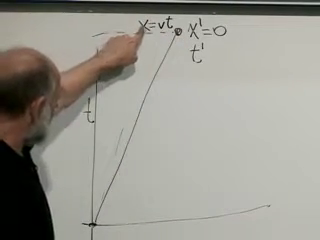
\includegraphics[width=0.72\textwidth]{lecture_04_figure_03.png}
\caption{Gốc chuyển động: $x=vt$, $x'=0$ và trục $t'$ là ba mô tả của cùng một đường thế giới.}
\lectureframe{00:48:18}
\end{figure}

Áp dụng khoảng bất biến giữa gốc chung và một điểm muộn hơn trên đường thế giới đó:
\begin{align}
t'^2-x'^2&=t^2-x^2,\\
t'^2&=t^2-v^2t^2,\\
t'&=t\sqrt{1-v^2}.
\label{eq:l4-time-dilation-natural}
\end{align}
Khi khôi phục $c$,
\begin{equation}
\Delta\tau=\Delta t\sqrt{1-\frac{v^2}{c^2}}
=\frac{\Delta t}{\gamma},
\qquad
\gamma=\frac{1}{\sqrt{1-v^2/c^2}}.
\label{eq:l4-time-dilation}
\end{equation}

\begin{figure}[H]
\centering
\includegraphics[width=0.73\textwidth]{lecture_04_figure_09.png}
\caption{Kết quả giãn thời gian trên bảng: đồng hồ chuyển động tích lũy $t'=t\sqrt{1-v^2}$ trong đơn vị với $c=1$.}
\lectureframe{00:50:45}
\end{figure}

Quan sát viên đứng yên nói rằng đồng hồ chuyển động chạy chậm. Tính tương hỗ đòi hỏi quan sát viên chuyển động cũng nói điều như vậy về các đồng hồ đứng yên. Không có mâu thuẫn nào, vì hai mô tả đang so sánh những cặp sự kiện ở xa khác nhau.

Thật vậy, một giá trị không đổi của $t'$ trong phương trình~\eqref{eq:l4-lorentz-natural} thỏa
\begin{equation}
t-vx=\text{constant}.
\label{eq:l4-simultaneity}
\end{equation}
Các đường đồng thời của quan sát viên chuyển động bị nghiêng so với các đường ngang $t=\text{constant}$. Mỗi quan sát viên gọi một tập hợp khác của các số chỉ đồng hồ ở xa là đồng thời. Một khi giữ rõ sự khác biệt đó, sự chạy chậm tương hỗ của các đồng hồ là nhất quán.

\begin{figure}[H]
\centering
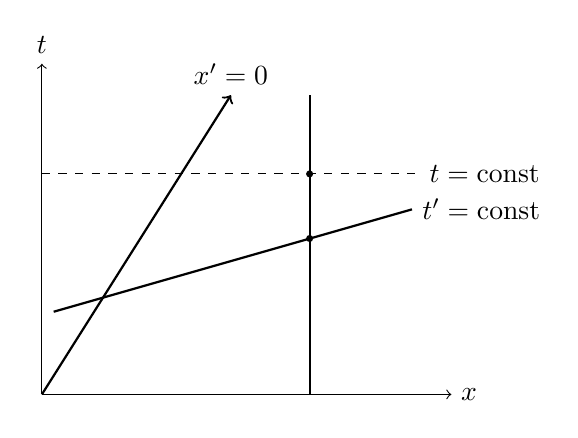
\begin{tikzpicture}[x=1cm,y=1cm]
\draw[->] (0,0) -- (0,4.2) node[above] {$t$};
\draw[->] (0,0) -- (5.2,0) node[right] {$x$};
\draw[thick,->] (0,0) -- (2.4,3.8) node[above] {$x'=0$};
\draw[dashed] (0,2.8) -- (4.8,2.8)
  node[right] {$t=\mathrm{const}$};
\draw[thick] (0.15,1.05) -- (4.7,2.35)
  node[right] {$t'=\mathrm{const}$};
\draw[thick] (3.4,0) -- (3.4,3.8);
\fill (3.4,2.8) circle (0.045);
\fill (3.4,1.98) circle (0.045);
\end{tikzpicture}
\caption{Sự giãn thời gian tương hỗ so sánh các số chỉ đồng hồ trên những lát cắt đồng thời khác nhau.}
\end{figure}

\section{Các quỹ đạo của cặp song sinh}

Hai người song sinh bắt đầu tại cùng một sự kiện. Một người ở lại tại $x=0$. Người kia đi ra xa với tốc độ $v$, đảo chiều, rồi trở về với cùng tốc độ ấy. Khi gặp lại nhau, họ so sánh mọi quá trình vật lý có thể đóng vai trò đồng hồ: đồng hồ đeo tay, nhịp tim, trao đổi chất, hay chính sự lão hóa.

Giả sử mỗi nửa chuyến đi kéo dài thời gian tọa độ $T$ trong hệ của người ở nhà. Thời gian riêng của người ở nhà là
\begin{equation}
\tau_{\mathrm{home}}=2T.
\end{equation}
Sự kiện quay đầu có tọa độ $(vT,T)$. Vì vậy chặng đi đầu đóng góp
\begin{align}
\tau_{\mathrm{leg}}
&=\sqrt{T^2-v^2T^2}
=T\sqrt{1-v^2}.
\end{align}
Chặng về đóng góp cùng một lượng, do đó
\begin{equation}
\tau_{\mathrm{travel}}=2T\sqrt{1-v^2}<2T.
\label{eq:l4-twin}
\end{equation}

\begin{figure}[H]
\centering
\includegraphics[width=0.73\textwidth]{lecture_04_figure_10.png}

\vspace{0.8em}

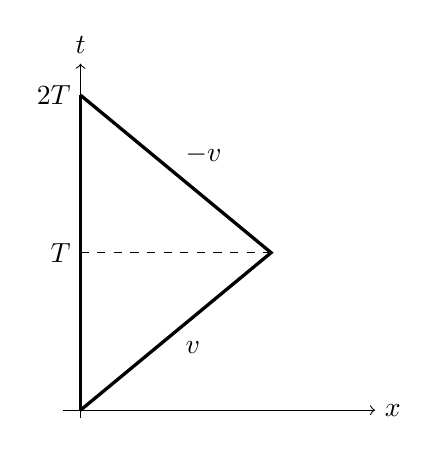
\begin{tikzpicture}[x=1.1cm,y=1cm]
\draw[->] (-0.2,0) -- (3.4,0) node[right] {$x$};
\draw[->] (0,-0.1) -- (0,4.4) node[above] {$t$};
\draw[very thick] (0,0) -- (0,4);
\draw[very thick] (0,0) -- (2.2,2) -- (0,4);
\draw[dashed] (0,2) -- (2.2,2);
\node[left] at (0,2) {$T$};
\node[left] at (0,4) {$2T$};
\node[below right] at (1.1,1.0) {$v$};
\node[above right] at (1.1,3.0) {$-v$};
\end{tikzpicture}
\caption{Đường thế giới của người ở nhà và hai chặng chuyển động. Thời gian riêng của chúng khác nhau vì chúng là những quỹ đạo khác nhau xuyên qua không-thời gian.}
\lectureframe{00:59:35}
\end{figure}

Không có mâu thuẫn nào trong việc tuổi tác không bằng nhau. Quỹ đạo chuyển động có một chỗ rẽ và không liên hệ với quỹ đạo thẳng của người ở nhà bởi một phép đối xứng của một hệ quy chiếu quán tính duy nhất. Trong hình học Euclid thông thường, một đường thẳng và một đường gãy giữa hai điểm cũng có độ dài khác nhau. Hình học Minkowski đảo ngược chuyện đường nào có khoảng lớn hơn, nhưng sự so sánh vẫn là hình học.

\section{Gia tốc và đồng hồ lý tưởng}

\begin{classroomqa}
\audiencequestion{Tại chỗ quay đầu, vật lý là khác đi và người du hành chịu gia tốc. Điều đó có làm mất hiệu lực của phép tính đồng hồ không?
\lecturetimestamp{01:02:19}}
\lecturerresponse{Gia tốc là có thật và giúp nhận diện tính bất đối xứng; không nên tìm cách gạt nó đi. Góc nhọn chỉ là một hình vẽ lý tưởng hóa và có thể được bo tròn thành một chỗ rẽ hữu hạn. Giả thiết vật lý bổ sung là một đồng hồ đủ nhỏ, chế tạo tốt sẽ không nhạy với gia tốc vừa phải và tiếp tục ghi thời gian riêng. Một đồng hồ lớn hoặc mong manh có thể bị biến dạng hay hỏng, nhưng đó là khuyết tật của cơ cấu chứ không phải của khoảng không-thời gian.}
\end{classroomqa}

Giả thiết đồng hồ lý tưởng này không được suy ra chỉ từ riêng phép biến đổi Lorentz. Nó được kiểm nghiệm thông qua ứng xử của các cơ cấu đồng hồ thực tế. Một nguyên tử là một xấp xỉ tốt hơn nhiều so với một chiếc đồng hồ rộng hàng trăm dặm, vì cơ cấu gọn nhỏ khó bị làm méo hơn dưới gia tốc hoặc trọng lực. Chỉ viện dẫn thuyết tương đối rộng bằng tên gọi cũng không loại bỏ được vấn đề vật lý này; người ta vẫn phải biết cơ cấu đã chọn đáp ứng với môi trường của nó như thế nào.

\begin{classroomqa}
\audiencequestion{Có thể chia một quỹ đạo gia tốc thành những khoảng ngắn mà trên đó phân tích quán tính vẫn còn đúng hay không?\lecturetimestamp{01:09:08}}
\lecturerresponse{Có. Hãy chia đường cong thành các đoạn ngắn, gần như thẳng, tính thời gian riêng trên từng đoạn rồi cộng các kết quả lại. Đây là phép tương tự trong không-thời gian của việc tìm độ dài của một đường cong thông thường từ nhiều đoạn thẳng nhỏ. Trong giới hạn liên tục,
\[
\tau=\int \sqrt{1-\frac{v(t)^2}{c^2}}\,dt,
\]
cho chuyển động trong không-thời gian phẳng được mô tả trong một hệ tọa độ quán tính.}
\end{classroomqa}

\section{Cặp song sinh thấy gì}

Có thể xác định bằng thao tác thực nghiệm các số đọc cuối cùng của đồng hồ bằng cách gửi các xung ánh sáng. Đánh dấu các khoảng 1 giây của thời gian riêng trên cả hai đường thế giới và cho mỗi người song sinh phát ra một xung ở mỗi mốc. Trong chặng đi ra xa, các xung nhận từ người kia thưa ra. Trong chặng quay về, chúng đến dồn lại. Đây là hiệu ứng Doppler tương đối tính được biểu diễn trực tiếp trên biểu đồ không-thời gian.

\begin{figure}[H]
\centering
\includegraphics[width=0.73\textwidth]{lecture_04_figure_11.png}
\caption{Các tín hiệu ánh sáng được trao đổi giữa đường thế giới của người ở nhà và của người du hành. Các tín hiệu đến thưa trong chặng đi ra xa và dồn lại trong chặng quay về vẫn tính đủ mọi xung được phát ra.}
\lectureframe{01:12:55}
\end{figure}

Không có hệ quy chiếu nào trong câu chuyện này biến mất. Mỗi người quan sát rốt cuộc đều nhận được tất cả các xung do người kia phát ra, nhưng tốc độ thu nhận của họ phụ thuộc vào chuyển động tương đối. Sự dịch đỏ trên chặng đi và sự dịch xanh trên chặng về không phải là các hiệu ứng kéo dài trong những khoảng thời gian bằng nhau trên hai chặng, nên việc đếm tất cả các xung nhận được phù hợp với phép so sánh thời gian riêng.

\begin{classroomqa}
\audiencequestion{Nếu người du hành quay về nhận ánh sáng bị dịch xanh, liệu người đó có thể thu được nhiều năng lượng hơn nguồn đã phát ra không?\lecturetimestamp{01:13:50}}
\lecturerresponse{Câu hỏi đó đòi hỏi định nghĩa tương đối tính về năng lượng và tính phụ thuộc hệ quy chiếu của nó, những điều chúng ta vẫn chưa trình bày. Đó là một câu hỏi hợp lý, nhưng chỉ riêng tọa độ và số đếm xung là không đủ để quyết định việc hạch toán năng lượng, đặc biệt đối với một người quan sát có gia tốc. Vì vậy nên hoãn câu trả lời lại thay vì đoán mò.}
\end{classroomqa}

\section{Một phương không gian khép kín}

\begin{classroomqa}
\audiencequestion{Giả sử một phương không gian là khép kín. Liệu một người song sinh có thể chuyển động đều theo phương ấy, trở về điểm xuất phát và hoàn toàn tránh được gia tốc không? Khi đó điều gì phân biệt hai người?\lecturetimestamp{01:15:14}}
\lecturerresponse{Không gian nên được hình dung một cách nội tại như một hình trụ, chứ không phải như một tấm bị uốn bên trong một không gian lớn hơn; không nhất thiết phải có gia tốc hướng tâm. Tuy vậy, người quan sát quay về vẫn đối mặt với sự kiện toàn cục rằng cùng một vị trí lặp lại. Điều đó cho thấy có một sự bất đối xứng, nhưng một câu trả lời đầy đủ đòi hỏi phải xử lý cẩn thận thuyết tương đối hẹp với phép đồng nhất hóa không gian này. Ở đây câu hỏi ấy được để ngỏ thay vì được trả lời ngẫu hứng.}
\end{classroomqa}

\begin{figure}[H]
\centering
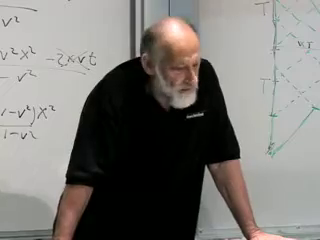
\includegraphics[width=0.72\textwidth]{lecture_04_figure_04.png}

\vspace{0.8em}

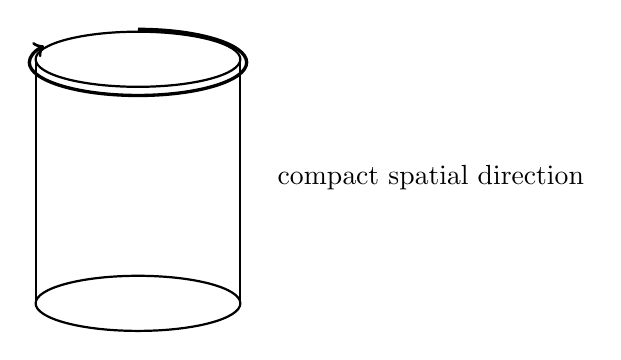
\begin{tikzpicture}[x=1cm,y=1cm]
\draw[thick] (0,0) ellipse (1.3 and 0.35);
\draw[thick] (-1.3,0) -- (-1.3,-3.1);
\draw[thick] (1.3,0) -- (1.3,-3.1);
\draw[thick] (0,-3.1) ellipse (1.3 and 0.35);
\draw[->,very thick] (0.0,0.38) arc (90:-210:1.38 and 0.42);
\node[right] at (1.65,-1.5) {compact spatial direction};
\end{tikzpicture}
\caption{Câu hỏi về không gian khép kín như được vẽ trên bảng, với một hình trụ nội tại thuần túy. Đây là một câu hỏi về phép đồng nhất hóa toàn cục, không phải về chuyển động quanh một hình trụ được nhúng trong một chiều hướng kính phụ thêm.}
\lectureframe{01:17:56}
\end{figure}

\section{Độ dài được đo trên một lát cắt đồng thời}

Đối với một bài toán trong thuyết tương đối hẹp, trước hết hãy vẽ bức tranh không-thời gian. Xét một thước mét đứng yên trong hệ không dấu phẩy, với hai đầu tại $x=0$ và $x=1$. Khi thời gian trôi đi, hai đầu ấy vạch nên các đường thế giới thẳng đứng. Cây thước quét ra một dải giữa chúng.

Người quan sát chuyển động phải đo cả hai đầu tại cùng một giá trị của thời gian $t'$ trong hệ chuyển động. Từ phương trình~\eqref{eq:l4-simultaneity}, lát cắt đi qua gốc tọa độ với $t'=0$ thỏa mãn \begin{equation}
t=vx
\end{equation} khi dùng đơn vị $c=1$. Nó cắt đầu bên phải $x=1$ tại $t=v$.

\begin{figure}[H]
\centering
\includegraphics[width=0.73\textwidth]{lecture_04_figure_12.png}

\vspace{0.8em}

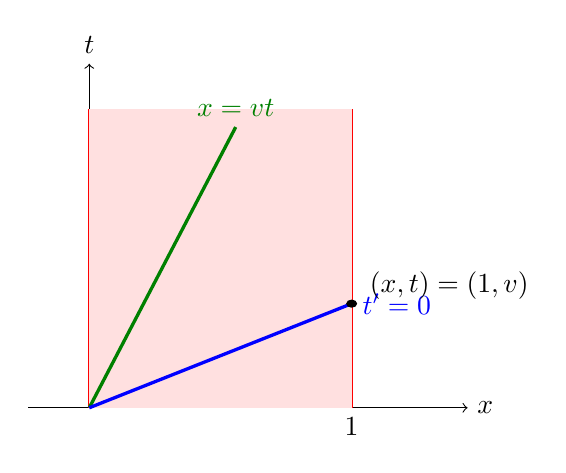
\begin{tikzpicture}[x=1.55cm,y=1.15cm]
\draw[->] (-0.5,0) -- (3.1,0) node[right] {$x$};
\draw[->] (0,0) -- (0,3.8) node[above] {$t$};
\draw[very thick,red] (0,0) -- (0,3.3);
\draw[very thick,red] (2.15,0) -- (2.15,3.3);
\fill[red!12] (0,0) rectangle (2.15,3.3);
\draw[very thick,green!50!black] (0,0) -- (1.2,3.1)
  node[above] {$x=vt$};
\draw[very thick,blue] (0,0) -- (2.15,1.15)
  node[right] {$t'=0$};
\fill (2.15,1.15) circle (0.045);
\node[right] at (2.22,1.35) {$(x,t)=(1,v)$};
\node[below] at (2.15,0) {$1$};
\end{tikzpicture}
\caption{Một thanh đứng yên quét ra một dải không-thời gian. Độ dài mà người quan sát chuyển động đo được là khoảng cách giữa hai đầu của nó trên một lát cắt $t'=\mathrm{const}$.}
\lectureframe{01:24:20}
\end{figure}

Độ tách giữa hai đầu được chọn là kiểu không gian, nên dùng dạng không gian mang dấu dương của bất biến:
\begin{equation}
x'^2-t'^2=x^2-t^2.
\end{equation}
Tại đầu mút được chọn, $t'=0$, $x=1$ và $t=v$. Do đó
\begin{align}
x'^2&=1-v^2,\\
x'&=\sqrt{1-v^2}.
\end{align}
Vì vậy, một độ dài riêng $L$ được đo trong hệ chuyển động là
\begin{equation}
L'=L\sqrt{1-v^2/c^2}=\frac{L}{\gamma}.
\label{eq:l4-length-contraction}
\end{equation}

\begin{figure}[H]
\centering
\includegraphics[width=0.76\textwidth]{lecture_04_figure_13.png}
\caption{Phép dựng hoàn chỉnh cho co độ dài và kết quả trên bảng $x'=\sqrt{1-v^2}$ đối với một độ dài riêng đơn vị.}
\lectureframe{01:28:10}
\end{figure}

Mệnh đề đối ứng cũng đúng: người quan sát trên sân ga gán một độ dài ngắn hơn cho thước mét theo phương dọc của đoàn tàu. Một lần nữa, hai người quan sát chọn những sự kiện đầu mút đồng thời khác nhau, nên tính đối ứng này không mâu thuẫn.

\section{Các câu hỏi ở phần cuối}

\begin{classroomqa}
\audiencequestion{Ngoài ánh sáng ra, có gì lan truyền với tốc độ ánh sáng không? Cụ thể, còn hấp dẫn thì sao?\lecturetimestamp{01:29:29}}
\lecturerresponse{Thuyết tương đối rộng dự đoán các sóng hấp dẫn lan truyền với $c$. Vào thời điểm của bài giảng này, bằng chứng chỉ đến gián tiếp từ các hệ như pulsar đôi; khi ấy sóng hấp dẫn vẫn chưa được phát hiện trực tiếp.\editorialnote{Tình hình thực nghiệm đã thay đổi sau bài giảng 2006 này. LIGO đã trực tiếp phát hiện GW150914 vào 2015, và việc quan sát đồng thời GW170817 cùng đối ứng điện từ của nó vào 2017 cho thấy tốc độ lan truyền của hấp dẫn và ánh sáng khớp nhau tới mức sai khác chỉ vài phần trên $10^{15}$. Xem \url{https://ligo.org/detections/gw150914/} và \url{https://doi.org/10.1103/PhysRevLett.119.251302}.}}
\end{classroomqa}

\begin{classroomqa}
\audiencequestion{Một phi hành gia có thể vượt qua một quãng đường dài nhiều năm ánh sáng trong một thời gian riêng nhỏ hơn giá trị của quãng đường đó khi biểu diễn bằng năm ánh sáng không? Điều đó có đồng nghĩa với chuyển động nhanh hơn ánh sáng không?\lecturetimestamp{01:30:38}}
\lecturerresponse{Thời gian riêng của phi hành gia là $\sqrt{\Delta t^2-\Delta x^2}$, nhỏ hơn thời gian tọa độ $\Delta t$. Trong hệ quán tính của phi hành gia, khoảng cách giữa các ngôi sao bị co Lorentz. Các ngôi sao chuyển động với vận tốc $-v$, chứ không nhanh hơn ánh sáng; đơn giản chỉ là khoảng cách đã co cần vượt qua nhỏ hơn.}
\end{classroomqa}

Nếu phi hành gia bắt đầu từ trạng thái đứng yên rồi gia tốc, mô tả sẽ thay đổi qua một chuỗi các hệ quán tính tức thời. Khoảng cách gán cho các ngôi sao có thể thay đổi trong quá trình chuyển tiếp đó. Không thể áp dụng một phép biến đổi Lorentz cố định cho toàn bộ lịch sử có gia tốc, nhưng tổng thời gian riêng vẫn được xác định bằng cách cộng các đóng góp dọc theo đường thế giới. Điều tương tự cũng áp dụng cho người song sinh trong tình huống thực tế, người phóng đi, quay đầu và giảm tốc, chứ không phải sinh ra đã ở tốc độ hành trình.

\begin{classroomqa}
\audiencequestion{Những điều khó hiểu này có phải do việc coi thời gian là đặc biệt không? Có nhất thiết phải gọi nó là chiều thứ tư không?\lecturetimestamp{01:36:43}}
\lecturerresponse{Không nhất thiết phải bắt đầu bằng khẩu hiệu rằng thời gian là chiều thứ tư. Chính phép biến đổi Lorentz buộc không gian và thời gian trộn lẫn, còn khoảng $t^2-x^2-y^2-z^2$ xem chúng như những phần của một hình học thống nhất với dấu khác nhau cho thời gian và không gian. Ở vận tốc thấp, sự trộn lẫn ấy trở nên không đáng kể và trực giác Newton quen thuộc quay trở lại. Tuy nhiên, ở vận tốc tương đối tính, không gian và thời gian không thể được xem là tách rời nhau một cách cơ bản.}
\end{classroomqa}

Vì vậy, sự giãn thời gian, co độ dài, việc so sánh hai người song sinh và thời gian hành trình rút ngắn không phải là những mẹo tách biệt. Tất cả đều theo từ ba thói quen: xác định các sự kiện đang được so sánh, vẽ hình học không-thời gian của chúng và dùng khoảng bất biến.